De resultaten van deze vraag zijn te vinden in Bijlage 1. In deze tabel staan de co\"effici\"entenvector x en het residu. Het is logisch dat het residu verkleint wanneer n stijgt. Er zijn meer vectoren u en dus is komt men steeds dichter bij een basis voor ${\rm I\!R}^{m}$. Het verhogen van n heeft steeds een kleiner effect, aangezien het bereik van alles vectoren samen slechts minimaal wordt vergroot. \\[12pt]

In de resultaten is dit gedrag zeer herkenbaar. We zien dat vanaf n = 23 elke verhoging van n slechts een verschil maakt van ongeveer 0.1. Dit is merkbaar kleiner dan de stappen ervoor die een verschil van eenheden of zelfs tientallen teweegbrengen. Merk wel dat het residu nog steeds zeer groot is. Dit is omdat er nog steed veel te weinig vectoren zijn ivm. de dimensie van het probleem nl. 400. Voor een n = 200 wordt het residu veel kleiner. Dan zijn er immer veel meer vectoren om een lineaire combinatie van te maken.\\[12pt]

Wanneer er echter gekeken wordt naar het effect van x op de benadering van de valideringsdata, treedt er een ander fenomeen op. Nu is er een minimum op n = 20. Dit valt te verklaren door het feit dat er op dat moment een nog niet zo specifieke oplossing is voor het probleem. Daarom is dit vage model nog toepasbaar op da valideerdata. Bij een hogere n worden de co\"effici\"enten een betere benadering van de modeldata, maar een minder goede voor de valideerdata.\\

\begin{figure}[H]
  \centering
  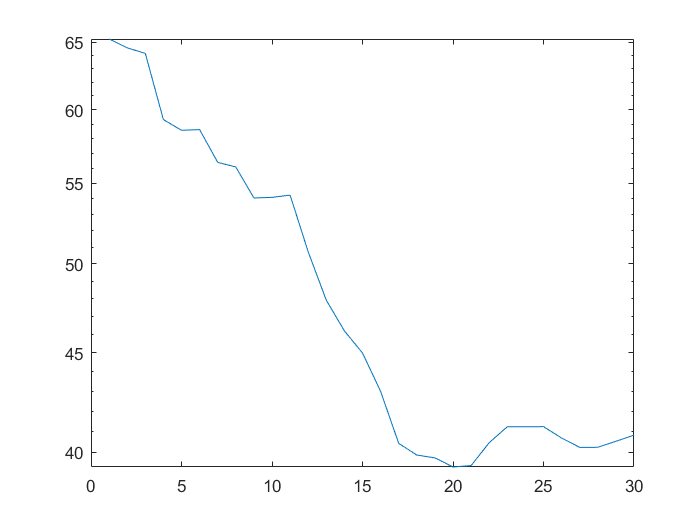
\includegraphics[width=0.5\textwidth]{Tekeningen/LeastSquare_Validate.png}
  \caption{Fout tussen model met u\_validate en x en y\_validate}
\end{figure}


